% !TEX TS-program = pdflatex
% !TEX encoding = UTF-8 Unicode

% This is a simple template for a LaTeX document using the "article" class.
% See "book", "report", "letter" for other types of document.

\documentclass[11pt]{article} % use larger type; default would be 10pt

\usepackage[utf8]{inputenc} % set input encoding (not needed with XeLaTeX)
\usepackage[document]{ragged2e}

%%% Examples of Article customizations
% These packages are optional, depending whether you want the features they provide.
% See the LaTeX Companion or other references for full information.

%%% PAGE DIMENSIONS
\usepackage{geometry} % to change the page dimensions
\geometry{a4paper} % or letterpaper (US) or a5paper or....
% \geometry{margin=2in} % for example, change the margins to 2 inches all round
% \geometry{landscape} % set up the page for landscape
%   read geometry.pdf for detailed page layout information

\usepackage[table,xcdraw]{xcolor}

\usepackage{graphicx} % support the \includegraphics command and options
\usepackage{enumerate}

% \usepackage[parfill]{parskip} % Activate to begin paragraphs with an empty line rather than an indent

%%% PACKAGES
\usepackage{booktabs} % for much better looking tables
\usepackage{array} % for better arrays (eg matrices) in maths
\usepackage{paralist} % very flexible & customisable lists (eg. enumerate/itemize, etc.)
\usepackage{verbatim} % adds environment for commenting out blocks of text & for better verbatim
\usepackage{subfig} % make it possible to include more than one captioned figure/table in a single float
% These packages are all incorporated in the memoir class to one degree or another...

%%% HEADERS & FOOTERS
\usepackage{fancyhdr} % This should be set AFTER setting up the page geometry
\pagestyle{fancy} % options: empty , plain , fancy
\renewcommand{\headrulewidth}{0pt} % customise the layout...
\lhead{}\chead{}\rhead{}
\lfoot{}\cfoot{\thepage}\rfoot{}

\usepackage{xcolor}

%%% SECTION TITLE APPEARANCE
\usepackage{sectsty}
\allsectionsfont{\sffamily\mdseries\upshape} % (See the fntguide.pdf for font help)
% (This matches ConTeXt defaults)

%%% ToC (table of contents) APPEARANCE
\usepackage[nottoc,notlof,notlot]{tocbibind} % Put the bibliography in the ToC
\usepackage[titles,subfigure]{tocloft} % Alter the style of the Table of Contents
\renewcommand{\cftsecfont}{\rmfamily\mdseries\upshape}
\renewcommand{\cftsecpagefont}{\rmfamily\mdseries\upshape} % No bold!
\usepackage{amsmath,amssymb}

%%% END Article customizations

%%% The "real" document content comes below...

\title{Métodos Determinísticos de Investigação Operacional \\ \large Trabalho Prático}
\author{Diogo Sobral, a82523 \\ Henrique Pereira, a80261 \\ Pedro Moreira, a82364 \\ Pedro Ferreira, a81135}
\date{2018/2019}

\begin{document}
\maketitle

\begin{figure*}[!b]
    \centering
    
\includegraphics[width=1in]{um_eeng.jpg}
\end{figure*}

\newpage

\section*{Contextualização}
Tendo em conta o anexo do enunciado, construimos uma tabela com os tempos de propagação do fogo entre os vários nodos, considerando que a não existência de uma ligação entre dois nodos implicaria que o seu tempo de propagação fosse 99999. Ora, para povoarmos esta tabela, corremos o script que apresentamos de seguida no programa IBM ILOG CPLEX Optimization Studio:
\begin{verbatim}
int a = ...;
int n = a*a;

int norte[1..a][1..a] = ...;
int este[1..a][1..a] = ...;
int sul[1..a][1..a] = ...;
int oeste[1..a][1..a] = ...;
 
int c[1..n][1..n];
execute {
      for(var i = 1; i<=n; i++) {
            for(var j = 1; j<=n; j++){
                  var dv = Opl.ceil(i/a);
                  var resto = i%a;
                  if(resto == 0) resto = a;

                  if((i-j) == a && dv!=1) c[i][j] = norte[dv][resto];
                  else if((i-j) == -1 && resto!=a) c[i][j] = este[dv][resto];
                  else if((i-j) == -a && dv!=a) c[i][j] = sul[dv][resto];
                  else if((i-j) == 1 && resto!=1) c[i][j] = oeste[dv][resto];
                  else c[i][j] = 99999;
                  }
            }
 }
\end{verbatim}
Neste caso, a é igual a 7 e as matrizes \texttt{norte},\texttt{este},\texttt{sul} e \texttt{oeste} contêm os custos de propagação do fogo entre dois nodos, consoante a direção do segundo relativamente ao primeiro, tendo em conta o anexo do enunciado.


Para o desenho dos grafos das soluções ótimas utilizamos a aplicação Web \textit{draw.io}.

\newpage

\section*{Questão 1}
\subsection*{a)}
\textbf{Parâmetros:}  \\
\begin{center}
n - número de nodos existentes \\
c\textsubscript{ij} - tempo de propagação no arco ij\\
i=1,...,n e j=1,...n \\
\end{center}
\textbf{Variáveis de Decisão:} \\
\begin{center}
X\textsubscript{ij} - número de caminhos a que o arco que une os nodos i e j pertence\\
i=1,...,n e j=1,...n \\
\end{center}
\textbf{Função Objetivo:} \\
$$min \ Z = \sum_{i=1}^{n} \sum_{j=1}^{n} c_i_jX_i_j$$
\textbf{Sujeito a:}
\begin{enumerate}[(i)]
\item $$\sum_{j=2}^{n} (X_1_j - X_j_1) = n-1$$
\item $$\sum_{j=1}^{n} (X_i_j - X_j_i) = -1, \forall i \in 2,...,n $$
\item $$X_i_j \geq 0, \forall i \in 1,...,n , \forall j \in 1,...,n$$
\end{enumerate}\\


Neste modelo, a função objetivo procura que o tempo de chegada do fogo a cada um dos nodos seja o mínimo possível pois serão considerados os arcos de menor custo. Uma vez que a variável de decisão representa o número de caminhos a que o arco ij pertence, o conjunto dos arcos com origem no nodo de ignição, ou seja, no nodo 1,  têm de necessariamente pertencer a todos os caminhos existentes. A restrição (i) expressa esta condição. Nos restantes nodos, o conjunto dos arcos com origem num determinado nodo i pertencem a menos um caminho que o conjunto dos nodos que chegam a i. Esta situação é definida pela restrição (ii). Por fim, a restrição (iii) estabelece a não negatividade das variáveis.
Aplicando este modelo geral à instância descrita no anexo do enunciado, temos o seguinte modelo de programação linear:

\newpage

\textbf{Variáveis de Decisão:} \\
\begin{center}
X\textsubscript{ij} - número de caminhos a que o arco que une os nodos i e j pertence\\
i=1,...,49 e j=1,...49 \\
\end{center}
\textbf{Função Objetivo:}
$$Min \ Z = 99999X_1_,_1 + 5X_1_,_2+99999X_1_,_3+...+3X_4_9_,_4_8+99999X_4_9_,_4_9$$
\textbf{Sujeito a:}
\begin{enumerate}[(i)]
\item $$(X_1_2-X_2_1)+(X_1_3-X_3_1)+...+(X_1_,_4_8-X_4_8_,_1)+(X_1_,_4_9-X_4_9_,_1)=48$$
\item $$(X_i_1-X_1_i)+(X_i_2-X_2_i)+...+(X_i_4_8-X_4_8_i)+(X_i_4_9-X_4_9_i)=-1, \forall i \in 2,...,49 $$
\item $$X_i_j \geq 0, \forall i \in 1,...,49, \forall j \in 1,...,49$$
\end{enumerate}\\

\subsection*{b)}

\textbf{Parâmetros:}
\begin{center}
n - número de nodos existentes \\
c\textsubscript{ij} - tempo de propagação no arco ij\\
i=1,...,n e j=1,...n \\
\end{center}
\textbf{Variáveis de Decisão:} \\
\begin{center}
T\textsubscript{i} - tempo decorrido desde a ignição aquando da chegada do fogo ao nodo i\\
i=1,...,n\\
\end{center}
\textbf{Função Objetivo:}
$$max \ Z = \sum_{i=1}^{n} T_i$$
\textbf{Sujeito a:}
\begin{enumerate}[(i)]
\item $$T_1 = 0$$
\item $$T_j \leq T_i + c_i_j, \forall i \in 1,...,n , \forall j \in 2,...,n$$
\item $$T_i \geq 0, \forall i \in 1,...,n$$
\end{enumerate}

Enquanto que o modelo primal tinha em consideração o número de caminhos a que um determinado arco pertencia, no modelo duas a variável de decisão representa o momento em que o fogo atinge um determinado nodo. Considerando a ignição no nodo 1, surge a restrição (i). Em conjunto com a função objetivo, a restrição (ii) garante que o tempo de chegada a cada nodo é o mínimo possível, tendo em conta a formulação do problema. Por um lado, queremos maximizar o tempo de chegada a cada nodo (função objetivo), por outro, pela restrição (ii), garante-se que o momento de chegada a um nodo j não é anterior ao menor dos tempos chegada ao conjunto dos nodos adjacentes a j, somado do custo de propagação para este. Por fim, a restrição (iii) estabelece a não negatividade das variáveis.

Aplicando o modelo geral à instância descrita no anexo do enunciado, temos o seguinte modelo de programação linear: \\
\textbf{Parâmetros:}  \\

\begin{center}
c\textsubscript{ij} - tempo de propagação no arco ij\\
i=1,...,n e j=1,...n \\
\end{center}
\textbf{Variáveis de Decisão:} \\
\begin{center}
T\textsubscript{i} - tempo decorrido desde a ignição aquando da chegada do fogo ao nodo i\\
i=1,...,49\\
\end{center}
\textbf{Função Objetivo:} \\
$$max \ Z = T_1+T_2+...+T_4_8+T_4_9$$
\textbf{Sujeito a:}
\begin{enumerate}[(i)]
\item $$T_1 = 0$$
\item $$T_j \leq T_i + c_i_j, \forall i \in 1,...,49 , \forall j \in 2,...,49$$
\item $$T_i \geq 0, \forall i \in 1,...,49$$
\end{enumerate}


\newpage

\subsection*{c)}
Solução ótima primal:

	\begin{figure}[!htpb]
		\centering
    		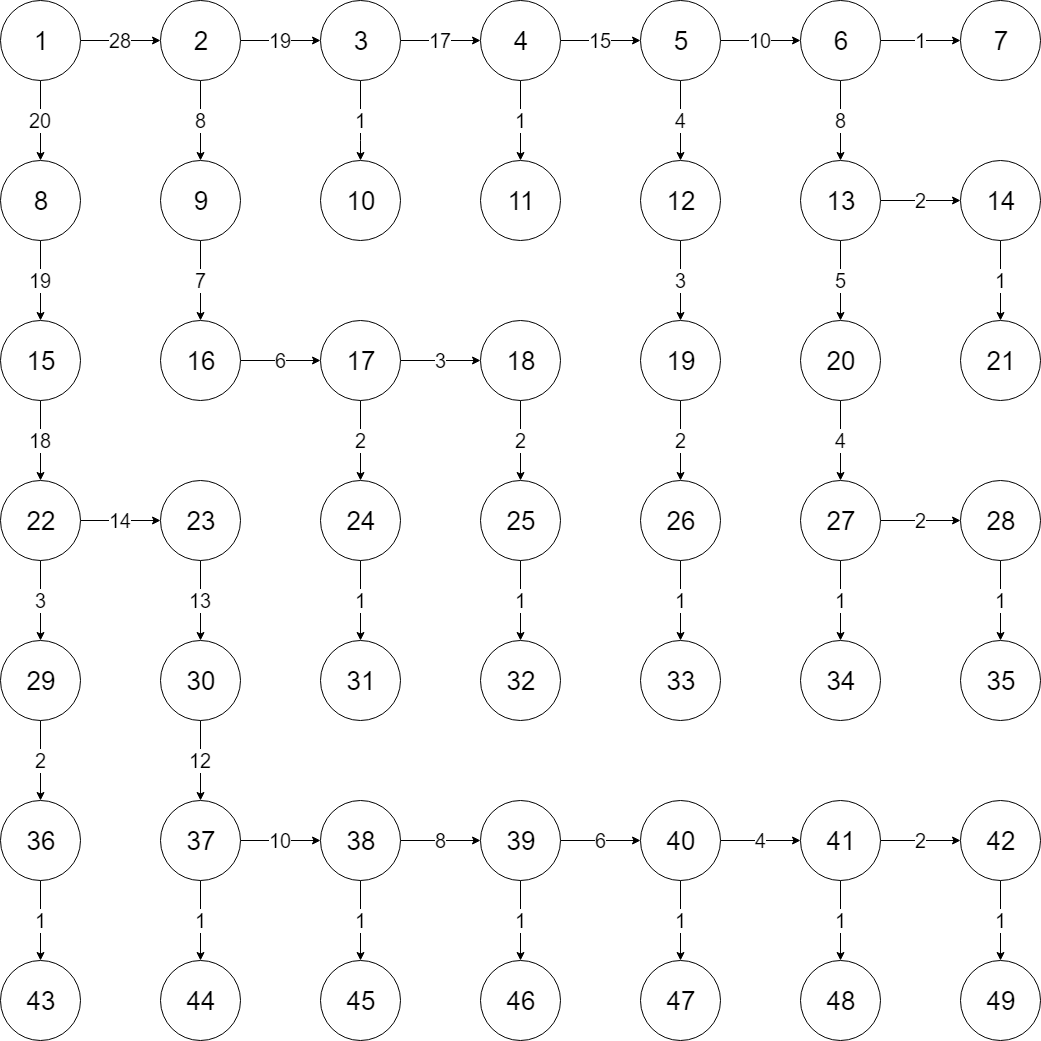
\includegraphics[width=5in]{grafo1c.png}
    		\caption{Representação gráfica da solução}
	\end{figure}


\textcolor{red}{Solução ótima dual:...}

\newpage

\subsection*{d)}
Solução ótima primal:

\begin{table}[h]
\centering
\begin{tabular}{lccccccc}
i/j                    & \multicolumn{1}{l}{1}            & \multicolumn{1}{l}{2}            & \multicolumn{1}{l}{3}            & \multicolumn{1}{l}{4}            & \multicolumn{1}{l}{5}            & \multicolumn{1}{l}{6}            & \multicolumn{1}{l}{7}            \\ \cline{2-8} 
\multicolumn{1}{l|}{1} & \multicolumn{1}{c|}{\textbf{0}}  & \multicolumn{1}{c|}{\textbf{5}}  & \multicolumn{1}{c|}{\textbf{10}} & \multicolumn{1}{c|}{\textbf{13}} & \multicolumn{1}{c|}{\textbf{16}} & \multicolumn{1}{c|}{\textbf{19}} & \multicolumn{1}{c|}{\textbf{22}} \\ \cline{2-8} 
\multicolumn{1}{l|}{2} & \multicolumn{1}{c|}{\textbf{7}}  & \multicolumn{1}{c|}{\textbf{12}} & \multicolumn{1}{c|}{\textbf{16}} & \multicolumn{1}{c|}{\textbf{20}} & \multicolumn{1}{c|}{\textbf{22}} & \multicolumn{1}{c|}{\textbf{25}} & \multicolumn{1}{c|}{\textbf{28}} \\ \cline{2-8} 
\multicolumn{1}{l|}{3} & \multicolumn{1}{c|}{\textbf{15}} & \multicolumn{1}{c|}{\textbf{18}} & \multicolumn{1}{c|}{\textbf{21}} & \multicolumn{1}{c|}{\textbf{26}} & \multicolumn{1}{c|}{\textbf{28}} & \multicolumn{1}{c|}{\textbf{32}} & \multicolumn{1}{c|}{\textbf{35}} \\ \cline{2-8} 
\multicolumn{1}{l|}{4} & \multicolumn{1}{c|}{\textbf{21}} & \multicolumn{1}{c|}{\textbf{24}} & \multicolumn{1}{c|}{\textbf{29}} & \multicolumn{1}{c|}{\textbf{32}} & \multicolumn{1}{c|}{\textbf{35}} & \multicolumn{1}{c|}{\textbf{38}} & \multicolumn{1}{c|}{\textbf{42}} \\ \cline{2-8} 
\multicolumn{1}{l|}{5} & \multicolumn{1}{c|}{\textbf{28}} & \multicolumn{1}{c|}{\textbf{30}} & \multicolumn{1}{c|}{\textbf{35}} & \multicolumn{1}{c|}{\textbf{39}} & \multicolumn{1}{c|}{\textbf{42}} & \multicolumn{1}{c|}{\textbf{46}} & \multicolumn{1}{c|}{\textbf{49}} \\ \cline{2-8} 
\multicolumn{1}{l|}{6} & \multicolumn{1}{c|}{\textbf{36}} & \multicolumn{1}{c|}{\textbf{36}} & \multicolumn{1}{c|}{\textbf{39}} & \multicolumn{1}{c|}{\textbf{42}} & \multicolumn{1}{c|}{\textbf{47}} & \multicolumn{1}{c|}{\textbf{50}} & \multicolumn{1}{c|}{\textbf{53}} \\ \cline{2-8} 
\multicolumn{1}{l|}{7} & \multicolumn{1}{c|}{\textbf{42}} & \multicolumn{1}{c|}{\textbf{4}}  & \multicolumn{1}{c|}{\textbf{46}} & \multicolumn{1}{c|}{\textbf{50}} & \multicolumn{1}{c|}{\textbf{54}} & \multicolumn{1}{c|}{\textbf{56}} & \multicolumn{1}{c|}{\textbf{60}} \\ \cline{2-8} 
\end{tabular}
\end{table}

Solução ótima dual:
	\begin{figure}[!htpb]
		\centering
    		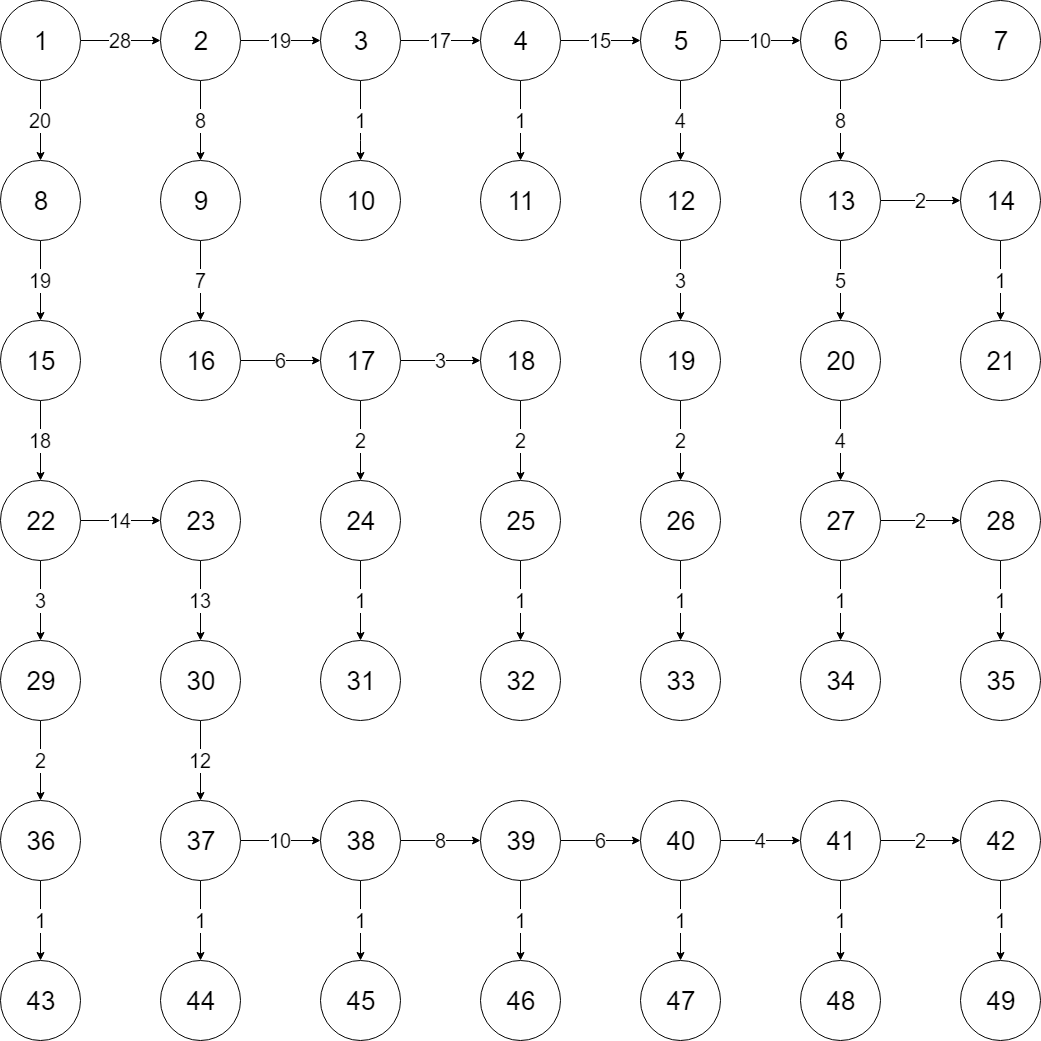
\includegraphics[width=5in]{grafo1c.png}
    		\caption{Representação gráfica da solução}
	\end{figure}

\newpage

\section*{Questão 2}
\subsection*{a)}
\textbf{Parâmetros:}  \\
\begin{center}
n - número de nodos existentes \\
Q\textsubscript{k} - Nodos adjacentes a k \\
k=1,...,n \\
c\textsubscript{ij} - tempo de propagação no arco ij\\
i=1,...,n e j=1,...n \\
b - número de recursos disponíveis \\
$\Delta$ - constante de retardação \\
ignição - célula de ignição do fogo \\
objetivo - célula a que se pretende atrasar a chegada do fogo
\end{center}

\textbf{Variáveis de Decisão:} \\
\begin{center}
X\textsubscript{i} = \begin{cases} 1, & \mbox{se é aplicado um recurso de proteção na célula i}  \\  0, & \mbox{caso contrário} \end{cases} \\
i=1,...,n \\
T\textsubscript{i} - tempo decorrido desde a ignição aquando da chegada do fogo ao nodo i \\
i=1,...,n \\
\end{center}
\textbf{Função Objetivo:} \\
$$max \ Z = T\textsubscript{$objetivo$}$$ \\

\textbf{Sujeito a:}
\begin{enumerate}[(i)]
\item $$T\textsubscript{ignição} = 0$$
\item $$T_j \leq T_i + c_i_j + \Delta * X_i, \forall i \in Q\textsubscript{j} , \forall j \in 1,...,n$$
\item $$\sum_{i=1}^{n} X_i \leq b$$
\item $$T_i \geq 0, \forall i \in 1,...,n$$
\end{enumerate}
O objetivo do problema é escolher onde aplicar recursos de proteção, que atrasam a propagação do fogo, de forma a retardar o máximo possível o momento de chegada do fogo a um determinado nodo (nodo objetivo). Para alcançar esse fim, consideramos como variável de decisão o tempo de chegada do fogo a cada nodo. Logo, a função objetivo procura maximizar o tempo de chegada ao nodo objetivo. Uma vez que a célula de ignição é um parâmetro do problema e não um valor fixo, temos de associar matematicamente o início do fogo ao nodo de ignição. A restrição (i) garante essa associação. A restrição (ii), em conjunto com a função objetivo, assegura a correta aplicação dos recursos de proteção, em função da célula que queremos proteger. Uma vez que o tempo de chegada do fogo a um certo nodo é definido por recorrência, isto é, o momento de chegada a um nodo j define-se à custa do tempo de chegada a outro nodo e assim sucessivamente até alcançarmos o nodo de ignição, único que se define a si mesmo, o modelo optará por colocar proteções em células que façam parte do caminho percorrido pelo fogo até ao nodo que queremos proteger, maximizando o tempo de chegada a este. A restrição(iii) limita o número de recursos aplicados e a restrição (iv) define a não negatividade das variáveis.
A função objetivo traduz a finalidade pretendida.
\subsection*{b)}
\begin{table}[h]
\centering
\begin{tabular}{cccccccc}
i/j                    & 1                                                        & 2                                                        & 3                                                        & 4                                & 5                                & 6                                                        & 7                                                        \\ \cline{2-8} 
\multicolumn{1}{c|}{1} & \multicolumn{1}{c|}{\cellcolor[HTML]{F8FF00}\textbf{0}}  & \multicolumn{1}{c|}{\cellcolor[HTML]{F8FF00}\textbf{13}} & \multicolumn{1}{c|}{\cellcolor[HTML]{F8FF00}\textbf{25}} & \multicolumn{1}{c|}{\textbf{36}} & \multicolumn{1}{c|}{\textbf{39}} & \multicolumn{1}{c|}{\textbf{42}}                         & \multicolumn{1}{c|}{\textbf{43}}                         \\ \cline{2-8} 
\multicolumn{1}{c|}{2} & \multicolumn{1}{c|}{\cellcolor[HTML]{F8FF00}\textbf{15}} & \multicolumn{1}{c|}{\cellcolor[HTML]{F8FF00}\textbf{27}} & \multicolumn{1}{c|}{\textbf{39}}                         & \multicolumn{1}{c|}{\textbf{41}} & \multicolumn{1}{c|}{\textbf{45}} & \multicolumn{1}{c|}{\textbf{48}}                         & \multicolumn{1}{c|}{\textbf{50}}                         \\ \cline{2-8} 
\multicolumn{1}{c|}{3} & \multicolumn{1}{c|}{\cellcolor[HTML]{F8FF00}\textbf{31}} & \multicolumn{1}{c|}{\textbf{41}}                         & \multicolumn{1}{c|}{\textbf{44}}                         & \multicolumn{1}{c|}{\textbf{49}} & \multicolumn{1}{c|}{\textbf{51}} & \multicolumn{1}{c|}{\textbf{55}}                         & \multicolumn{1}{c|}{\textbf{57}}                         \\ \cline{2-8} 
\multicolumn{1}{c|}{4} & \multicolumn{1}{c|}{\textbf{45}}                         & \multicolumn{1}{c|}{\textbf{48}}                         & \multicolumn{1}{c|}{\textbf{52}}                         & \multicolumn{1}{c|}{\textbf{55}} & \multicolumn{1}{c|}{\textbf{58}} & \multicolumn{1}{c|}{\textbf{61}}                         & \multicolumn{1}{c|}{\textbf{65}}                         \\ \cline{2-8} 
\multicolumn{1}{c|}{5} & \multicolumn{1}{c|}{\textbf{52}}                         & \multicolumn{1}{c|}{\textbf{54}}                         & \multicolumn{1}{c|}{\textbf{57}}                         & \multicolumn{1}{c|}{\textbf{62}} & \multicolumn{1}{c|}{\textbf{65}} & \multicolumn{1}{c|}{\textbf{69}}                         & \multicolumn{1}{c|}{\textbf{72}}                         \\ \cline{2-8} 
\multicolumn{1}{c|}{6} & \multicolumn{1}{c|}{\textbf{57}}                         & \multicolumn{1}{c|}{\textbf{60}}                         & \multicolumn{1}{c|}{\textbf{63}}                         & \multicolumn{1}{c|}{\textbf{66}} & \multicolumn{1}{c|}{\textbf{71}} & \multicolumn{1}{c|}{\textbf{74}}                         & \multicolumn{1}{c|}{\cellcolor[HTML]{F8FF00}\textbf{77}} \\ \cline{2-8} 
\multicolumn{1}{c|}{7} & \multicolumn{1}{c|}{\textbf{59}}                         & \multicolumn{1}{c|}{\textbf{64}}                         & \multicolumn{1}{c|}{\textbf{69}}                         & \multicolumn{1}{c|}{\textbf{73}} & \multicolumn{1}{c|}{\textbf{77}} & \multicolumn{1}{c|}{\cellcolor[HTML]{F8FF00}\textbf{80}} & \multicolumn{1}{c|}{\cellcolor[HTML]{32CB00}\textbf{92}} \\ \cline{2-8} 
\end{tabular}
\caption{Representação gráfica da rede de nodos com os tempos da solução obtida.}
\end{table}
\begin{itemize}[$\ast$]
    \item As células a branco representam nodos normais.
    \item As células a amarelo representam os nodos onde foram gastos os recursos.
    \item A célula a verde é o nodo a ser protegido.
\end{itemize}
\par Durante o teste deste modelo, deparamo-nos diversas vezes com valores do tempo de chegada do fogo a certas células que eram difíceis de explicar, especialmente quando eram usados poucos recursos. Estes valores levantaram alguma confusão, uma vez que os tempos de chegada do fogo a essas células eram menores do que o suposto. Após vários testes para verificar a robustez do modelo, chegamos à conclusão que os tempos de chegada do fogo a um nodo apenas estavam corretos para aqueles que contribuíam para a solução do problema. Tal acontece pois só são maximizados os tempos de chegada aos nodos que fazem parte do percurso que o fogo realiza até atingir a célula que queremos proteger. De facto, pela função objetivo, estamos a maximizar não só o tempo de chegada à célula objetivo, mas também às restantes que fazem parte do percurso até essa célula, uma vez que a restrição (ii) tem caráter recursivo.
\subsection*{c)}
\begin{figure*}[h]
    \centering
    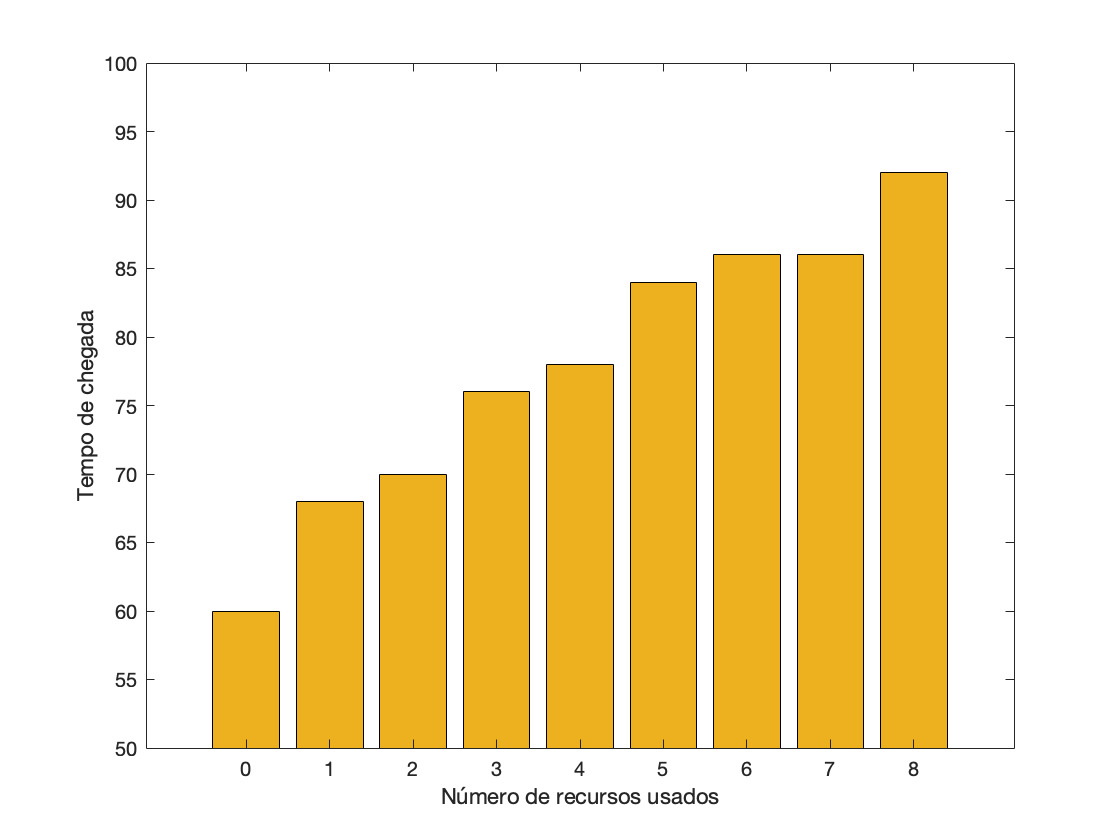
\includegraphics[scale=0.3]{graf2.png}
    \caption{Gráfico Recursos usados - Tempo de chegada}
\end{figure*}

\par Na figura 1 está representado um gráfico que faz uma associação entre o número de recursos utilizados na proteção e o respetivo tempo de chegada à célula (7,7) (nodo nº 49). Para esta experiência, consideramos o número de recursos disponíveis entre 0 e 8. Como seria expectável, quanto maior o número de recursos disponíveis, mais tarde o fogo atinge a célula objetivo. Inicialmente, sem aplicação de recursos de proteção, o tempo de chegada está situado em 60 e, à medida que aplicamos recursos, varia até 92. As maiores subidas dão-se quando são utilizados  1,5,8 recursos. É de notar que a aplicação de um recurso, neste caso, nunca resulta num incremento do tempo de chegada em 12 unidades de tempo (valor $\Delta$), o que indica a ocorrência de uma mudança no percurso utilizado para atingir a célula objetivo, perante a aplicação de um recurso de proteção.

\newpage

\section*{Questão 3}

\subsection*{a)}
\textbf{Parâmetros:}  \\
\begin{center}
n - número de nodos existentes \\
c\textsubscript{ij} - tempo de propagação no arco ij\\
i=1,...,n e j=1,...n \\
t\textsubscript{max} - intervalo de tempo considerado\\
b - número de recursos disponíveis \\
$\Delta$ - constante de retardação \\
p\textsubscript{s} - probabilidade de ignição na célula s\\
s=1,...n \\
\end{center}
\textbf{Variáveis de Decisão:} \\

\begin{center}
X\textsubscript{i} = \begin{cases} 1, & \mbox{se é aplicado um recurso de proteção no nodo i}\\ 0, & \mbox{caso contrário}\end{cases} \\
i=1,...,n \\
T\textsubscript{si} - tempo decorrido aquando da chegada de um fogo, com origem em s, ao nodo i\\
s=1,...,n e i=1,...,n \\
Y\textsubscript{si} = \begin{cases} 1, & \mbox{se o fogo com início no nodo} \ s \ \mbox{chega a} \ i \  \mbox{num tempo inferior a t\textsubscript{max}} \\ 0, & \mbox{caso contrário}\end{cases} \\
s=1,...,n e i=1,...,n
\end{center}

\textbf{Função Objetivo:} \\
$$min \ Z = \sum_{s=1}^{n} \sum_{i=1}^{n} p_sY_s_i$$ \\


\textbf{Sujeito a:}
\begin{enumerate}[(i)]
\item $$T\textsubscript{ss} = 0, \forall s \in 1,...,n$$
\item $$T_s_j \leq T_s_i + d_i_j + \Delta X_i, \forall s \in 1,...n, \forall i \in 1,...,n , \forall j \in 1,...,n$$
\item $$Y_s_i \geq \frac{ t\textsubscript{max}-T_s_i}{t\textsubscript{max}}, \forall s \in 1,...,n, \forall i \in 1,...,n $$
\item $$\sum_{i=1}^{n} X_i \leq b$$
\end{enumerate}

O objetivo deste problema é escolher onde aplicar recursos de proteção de forma a minimizar o valor esperado de área ardida, dada a probabilidade de ignição em cada nodo. A resolução deste problema é semelhante à do problema anterior, onde queríamos proteger uma determinada célula. Neste caso, queremos proteger o maior número de células possíveis, consoante o ponto de ignição. Deste modo, introduzimos uma nova variável de decisão, Y\textsubscript{si}, que representa o facto de uma célula arder ou não, considerando um período de tempo, e um nodo de ignição do fogo. O objetivo passa por minimizar  o número de células que arderiam se o fogo começasse num nodo s.
Para obtermos o valor esperado de área ardida, multiplicamos a probabilidade de ignição em s pelo número de células que seriam afetados por um fogo com início nesse nodo. A função objetivo tenta então minimizar o valor obtido pela repetição do cenário descrito em cada um dos nodos existentes. A restrição (i) força o tempo de chegada do fogo ao ponto de ignição a ser zero. A restrição (ii) impede que o tempo de chegada do fogo a um nodo seja inferior que o menor tempo de chegada a um adjacente, somado do tempo de propagação. A restrição (iii), em conjunto com a função objetivo, faz com o que tempo de chegada do fogo a um nodo seja maximizado (enquanto este for inferior a t\textsubscript{max}). Uma vez que queremos minimizar Y\textsubscript{si}, temos que aumentar o valor de T\textsubscript{si}. Se  T\textsubscript{si} for igual ou superior a t\textsubscript{max} então o lado direito da restrição (iii) é um valor negativo, pelo que teremos Y\textsubscript{si}=0, pois estamos a minimizar o seu valor. Este cenário significa que a célula i não arde se o fogo começar em s. Por outro lado, se T\textsubscript{si} for menor que  t\textsubscript{max} a célula vai arder. Efetivamente, o lado direito da restrição (iii) será um valor positivo, menor ou igual a um e superior a zero, pelo que Y\textsubscript{si} só poderá ter valor igual a um. A restrição (iv) limita o número de recursos aplicados.
\subsection*{b)}

\begin{table}[h]
\centering
\begin{tabular}{cccccccc}
i/j                    & 1                                                       & 2                                                       & 3                                                       & 4                                                       & 5                                                       & 6                                                       & 7                                                        \\ \cline{2-8} 
\multicolumn{1}{c|}{1} & \multicolumn{1}{c|}{\cellcolor[HTML]{FFFFFF}\textbf{4}} & \multicolumn{1}{c|}{\cellcolor[HTML]{FFFFFF}\textbf{5}} & \multicolumn{1}{c|}{\cellcolor[HTML]{F8FF00}\textbf{2}} & \multicolumn{1}{c|}{\cellcolor[HTML]{FFFFFF}\textbf{4}} & \multicolumn{1}{c|}{\cellcolor[HTML]{F8FF00}\textbf{3}} & \multicolumn{1}{c|}{\cellcolor[HTML]{FFFFFF}\textbf{6}} & \multicolumn{1}{c|}{\cellcolor[HTML]{FFFFFF}\textbf{5}}  \\ \cline{2-8} 
\multicolumn{1}{c|}{2} & \multicolumn{1}{c|}{\cellcolor[HTML]{FFFFFF}\textbf{4}} & \multicolumn{1}{c|}{\cellcolor[HTML]{F8FF00}\textbf{2}} & \multicolumn{1}{c|}{\cellcolor[HTML]{FFFFFF}\textbf{5}} & \multicolumn{1}{c|}{\cellcolor[HTML]{F8FF00}\textbf{1}} & \multicolumn{1}{c|}{\cellcolor[HTML]{FFFFFF}\textbf{8}} & \multicolumn{1}{c|}{\cellcolor[HTML]{FFFFFF}\textbf{8}} & \multicolumn{1}{c|}{\cellcolor[HTML]{FFFFFF}\textbf{7}}  \\ \cline{2-8} 
\multicolumn{1}{c|}{3} & \multicolumn{1}{c|}{\cellcolor[HTML]{FFFFFF}\textbf{6}} & \multicolumn{1}{c|}{\cellcolor[HTML]{FFFFFF}\textbf{8}} & \multicolumn{1}{c|}{\cellcolor[HTML]{FFFFFF}\textbf{6}} & \multicolumn{1}{c|}{\cellcolor[HTML]{F8FF00}\textbf{1}} & \multicolumn{1}{c|}{\cellcolor[HTML]{FFFFFF}\textbf{8}} & \multicolumn{1}{c|}{\cellcolor[HTML]{FFFFFF}\textbf{8}} & \multicolumn{1}{c|}{\cellcolor[HTML]{FFFFFF}\textbf{7}}  \\ \cline{2-8} 
\multicolumn{1}{c|}{4} & \multicolumn{1}{c|}{\cellcolor[HTML]{FFFFFF}\textbf{6}} & \multicolumn{1}{c|}{\cellcolor[HTML]{FFFFFF}\textbf{5}} & \multicolumn{1}{c|}{\cellcolor[HTML]{F8FF00}\textbf{2}} & \multicolumn{1}{c|}{\cellcolor[HTML]{FFFFFF}\textbf{8}} & \multicolumn{1}{c|}{\cellcolor[HTML]{FFFFFF}\textbf{8}} & \multicolumn{1}{c|}{\cellcolor[HTML]{FFFFFF}\textbf{9}} & \multicolumn{1}{c|}{\cellcolor[HTML]{FFFFFF}\textbf{6}}  \\ \cline{2-8} 
\multicolumn{1}{c|}{5} & \multicolumn{1}{c|}{\cellcolor[HTML]{FFFFFF}\textbf{5}} & \multicolumn{1}{c|}{\cellcolor[HTML]{F8FF00}\textbf{1}} & \multicolumn{1}{c|}{\cellcolor[HTML]{FFFFFF}\textbf{6}} & \multicolumn{1}{c|}{\cellcolor[HTML]{FFFFFF}\textbf{8}} & \multicolumn{1}{c|}{\cellcolor[HTML]{FFFFFF}\textbf{9}} & \multicolumn{1}{c|}{\cellcolor[HTML]{FFFFFF}\textbf{8}} & \multicolumn{1}{c|}{\cellcolor[HTML]{FFFFFF}\textbf{6}}  \\ \cline{2-8} 
\multicolumn{1}{c|}{6} & \multicolumn{1}{c|}{\cellcolor[HTML]{FFFFFF}\textbf{6}} & \multicolumn{1}{c|}{\cellcolor[HTML]{FFFFFF}\textbf{6}} & \multicolumn{1}{c|}{\cellcolor[HTML]{F8FF00}\textbf{2}} & \multicolumn{1}{c|}{\cellcolor[HTML]{FFFFFF}\textbf{7}} & \multicolumn{1}{c|}{\cellcolor[HTML]{FFFFFF}\textbf{9}} & \multicolumn{1}{c|}{\cellcolor[HTML]{FFFFFF}\textbf{8}} & \multicolumn{1}{c|}{\cellcolor[HTML]{FFFFFF}\textbf{7}}  \\ \cline{2-8} 
\multicolumn{1}{c|}{7} & \multicolumn{1}{c|}{\cellcolor[HTML]{FFFFFF}\textbf{4}} & \multicolumn{1}{c|}{\cellcolor[HTML]{FFFFFF}\textbf{5}} & \multicolumn{1}{c|}{\cellcolor[HTML]{FFFFFF}\textbf{6}} & \multicolumn{1}{c|}{\cellcolor[HTML]{FFFFFF}\textbf{7}} & \multicolumn{1}{c|}{\cellcolor[HTML]{FFFFFF}\textbf{6}} & \multicolumn{1}{c|}{\cellcolor[HTML]{FFFFFF}\textbf{5}} & \multicolumn{1}{c|}{\cellcolor[HTML]{FFFFFF}\textbf{49}} \\ \cline{2-8} 
\end{tabular}
\caption{Representação da solução ótima}
\end{table}

\begin{itemize}[$\ast$]
	\item As células a amarelo representam os nodos onde foram gastos os recursos.
    \item As células a branco são nodos normais.
\end{itemize}
A tabela 2 apresenta uma das representações gráficas da solução do problema. A cada célula está associado um valor que representa a área ardida caso o nodo de ignição seja o mesmo. As células pintadas a amarelo são os locais onde foram utilizados os recursos. Pela análise dos valores, concluímos que os valores mais baixos estão situados nos locais onde são alocados os recursos. A célula 7,7 tem o valor 49 que, neste caso, é um valor descontextualizado visto que, como a sua probabilidade de ignição é 0, este nodo nunca começará o fogo logo o valor da área ardida é indiferente.

\begin{table}[h]
\centering
\begin{tabular}{cccccccc}
i\textbackslash{}j     & 1                                   & 2                                   & 3                                   & 4                                   & 5                                   & 6                                   & 7                                   \\ \cline{2-8}
\multicolumn{1}{c|}{1} & \multicolumn{1}{c|}{\textbf{0.068}} & \multicolumn{1}{c|}{\textbf{0.046}} & \multicolumn{1}{c|}{\textbf{0.102}} & \multicolumn{1}{c|}{\textbf{0.06}}  & \multicolumn{1}{c|}{\textbf{0.078}} & \multicolumn{1}{c|}{\textbf{0.056}} & \multicolumn{1}{c|}{\textbf{0.036}} \\ \cline{2-8}
\multicolumn{1}{c|}{2} & \multicolumn{1}{c|}{\textbf{0.108}} & \multicolumn{1}{c|}{\textbf{0.1}}   & \multicolumn{1}{c|}{\textbf{0.034}} & \multicolumn{1}{c|}{\textbf{0.088}} & \multicolumn{1}{c|}{\textbf{0.062}} & \multicolumn{1}{c|}{\textbf{0.072}} & \multicolumn{1}{c|}{\textbf{0.07}}  \\ \cline{2-8}
\multicolumn{1}{c|}{3} & \multicolumn{1}{c|}{\textbf{0.094}} & \multicolumn{1}{c|}{\textbf{0.07}}  & \multicolumn{1}{c|}{\textbf{0.072}} & \multicolumn{1}{c|}{\textbf{0.104}} & \multicolumn{1}{c|}{\textbf{0.066}} & \multicolumn{1}{c|}{\textbf{0.074}} & \multicolumn{1}{c|}{\textbf{0.058}} \\ \cline{2-8}
\multicolumn{1}{c|}{4} & \multicolumn{1}{c|}{\textbf{0.088}} & \multicolumn{1}{c|}{\textbf{0.072}} & \multicolumn{1}{c|}{\textbf{0.124}} & \multicolumn{1}{c|}{\textbf{0.072}} & \multicolumn{1}{c|}{\textbf{0.066}} & \multicolumn{1}{c|}{\textbf{0.072}} & \multicolumn{1}{c|}{\textbf{0.046}} \\ \cline{2-8}
\multicolumn{1}{c|}{5} & \multicolumn{1}{c|}{\textbf{0.048}} & \multicolumn{1}{c|}{\textbf{0.098}} & \multicolumn{1}{c|}{\textbf{0.042}} & \multicolumn{1}{c|}{\textbf{0.066}} & \multicolumn{1}{c|}{\textbf{0.076}} & \multicolumn{1}{c|}{\textbf{0.04}}  & \multicolumn{1}{c|}{\textbf{0.034}} \\ \cline{2-8}
\multicolumn{1}{c|}{6} & \multicolumn{1}{c|}{\textbf{0.054}} & \multicolumn{1}{c|}{\textbf{0.052}} & \multicolumn{1}{c|}{\textbf{0.07}}  & \multicolumn{1}{c|}{\textbf{0.054}} & \multicolumn{1}{c|}{\textbf{0.048}} & \multicolumn{1}{c|}{\textbf{0.04}}  & \multicolumn{1}{c|}{\textbf{0.03}}  \\ \cline{2-8}
\multicolumn{1}{c|}{7} & \multicolumn{1}{c|}{\textbf{0.062}} & \multicolumn{1}{c|}{\textbf{0.062}} & \multicolumn{1}{c|}{\textbf{0.04}}  & \multicolumn{1}{c|}{\textbf{0.044}} & \multicolumn{1}{c|}{\textbf{0.3}}   & \multicolumn{1}{c|}{\textbf{0.024}} & \multicolumn{1}{c|}{\textbf{0.012}} \\ \cline{2-8}
\end{tabular}
\caption{Probabilidade da céluda arder}
\end{table}

Ao contrário da tabela 2 em que a interpretação da solução se baseava na área ardida provocada pela ignição de um nodo, a tabela 3 apresenta a probabilidade de um nodo arder. A probabilidade de um nodo arder é dada pela soma das probabilidades de ignição de todos os nodos à sua volta em que o fogo chega ao nodo desejado num intervalo de tempo menor que o pretendido. Assim sabendo que nodos ardem provocados pela ignição de outro nodo conseguimos prever a probabilidade de um dado nodo arder antes do tempo.
\newpage
\subsection*{c)}
\begin{figure*}[h]
    \centering
    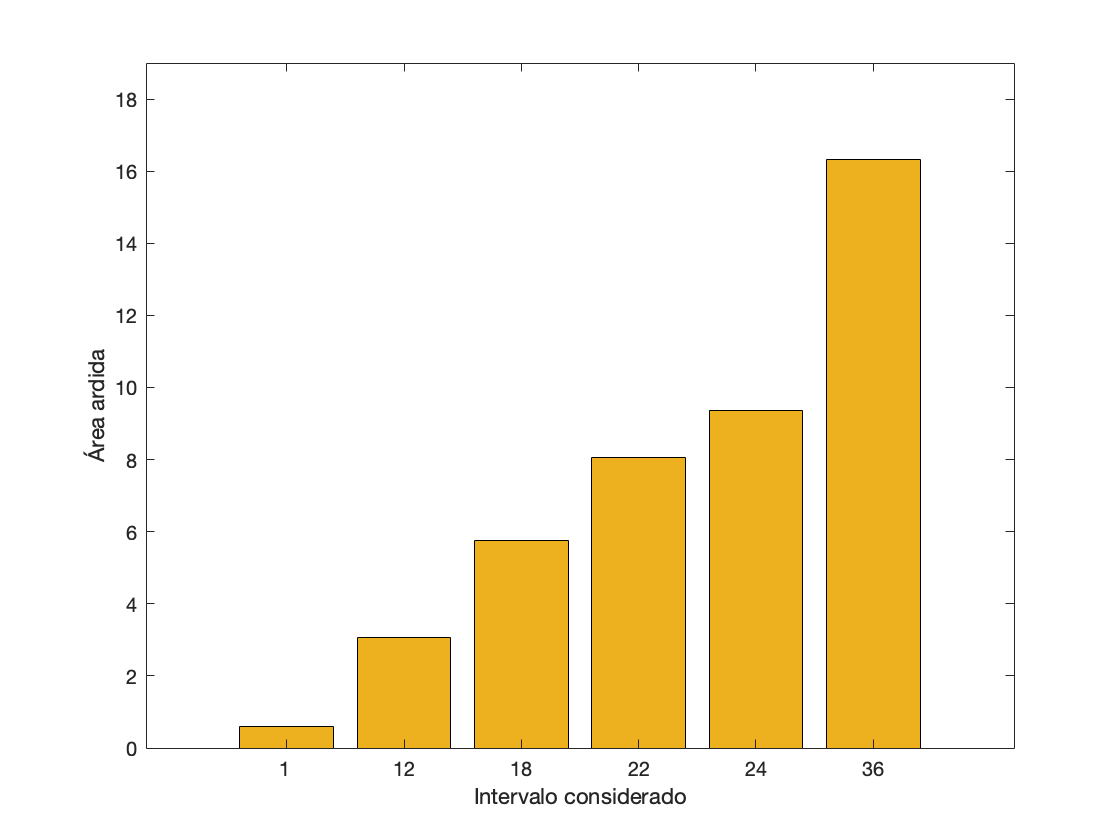
\includegraphics[scale=0.3]{graf3.png}
    \caption{Gráfico Tempo considerado - Área Ardida}
\end{figure*}

A figura 3 estabelece um correspondência entre a tmax utilizado e o a área ardida. Os valores correspondem a amostras que corremos no nosso modelo e que foram mais tarde utilizados para a construção do gráfico. O intervalo de tempo mais pequeno que consideramos foi o 1. Inicialmente, era expectável que para um intervalo tão pequeno a área ardida não fosse menor que 1 (local onde o fogo começa). No entanto, como existe a possibilidade de não haver fogo, a área ardida pode tomar valores inferiores, mas nunca inferiores a 0. À medida que o tempo aumenta, a área ardida também aumenta, numa fase inicial, até serem considerados intervalos de tempo muito grandes em que a área esperada estagne ou atinja valores muito próximos de 49 (tudo ardido). Infelizmente, não conseguimos arranjar valores que suportem o que afirmamos, uma vez que o tempo de cálculo do OPL cresce em tempo exponencial e ,se para tmax = 36, a solução ótima demorou 30 minutos a ser calculada. Assim, para valores de tmax, em que arde tudo, iria, certamente, demorar horas, tornando a situação impraticável.

\end{document}
